%\documentclass[12pt,serif]{beamer}
%\documentclass[tikz,12pt,svgnames]{beamer}
\documentclass[table,handout,tikz,12pt,svgnames]{beamer}
\usepackage{CM-preamble}
\subtitle{\LARGE Listes chaînées : variantes}
\date{CM6}

%README TODO STUFF

\begin{document}

\begin{frame}
	\titlepage
\end{frame}

\begin{frame}[fragile=singleslide]
	\frametitle{Listes chaînées : variantes}
		\begin{block}{Maintenir la longueur}
			\begin{itemize}
				\item Pour accès par position : \texttt{ k < longueur(L)}
			\end{itemize}
		\end{block}
		\begin{block}{Maintenir un pointeur sur la dernière cellule}
			\begin{itemize}
				\item Accès et modifications courantes en queue
			\end{itemize}
		\end{block}
		\begin{block}{Introduction d'une tête fictive}
			\begin{itemize}
				\item Pour simplifier ajout / suppression en tête
			\end{itemize}
		\end{block}
%		\IMAGE
%		{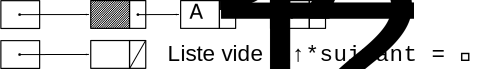
\includegraphics[scale=0.6]{../common-images/liste_variantes1.pdf}}
	\begin{center}
			{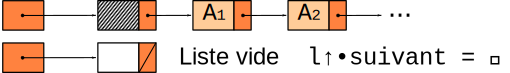
\includegraphics[scale=0.7]{../common-images/liste_variantes1_color.pdf}}
	\end{center}
\end{frame}


\begin{frame}[fragile=singleslide]
	\frametitle{Listes symétriques \large (ou doublement chaînées)}
	\begin{block}{}
		\begin{itemize}
			\item Facilitent parcours symétriques (dans les 2 sens)
			\item Ajout/retrait sans nécessiter le \texttt{prec}
%			\item \IMAGE
		\end{itemize}
		\vspace{-2em}
		\begin{center}
			{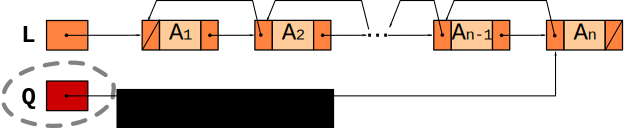
\includegraphics[scale=0.7]{../common-images/liste_variantes2_color.pdf}}
		\end{center}
	\end{block}
	\vspace{-1cm}
	\begin{block}{}
		\begin{minted}[mathescape=true,escapeinside=||]{text}
|\underline{Action}| supp(P)
	|\underline{D/R}| : P : Liste_contiguë
	P|$\uparrow\bullet$|prec|$\uparrow\bullet$|suiv| $\leftarrow$| P|$\uparrow\bullet$|suiv
	P|$\uparrow\bullet$|suiv|$\uparrow\bullet$|prec| $\leftarrow$| P|$\uparrow\bullet$|prec
	libérer (P)
|\underline{Faction}|
		\end{minted}
	\end{block}
%	\begin{block}{}
%		\begin{minted}[mathescape=true,escapeinside=||]{text}
%		|\underline{Action}| affich(l)
%		|\underline{D}| : l : Liste_contiguë 
%		|\underline{L}| : i : Entier
%		|\underline{Pour}| i de 0 à l.dernier |\underline{Faire}|
%		ecrire(l.espace[i])
%		|\underline{Fpour}|
%		|\underline{Faction}|
%		\end{minted}
%	\end{block}
\end{frame}


\begin{frame}[fragile=singleslide]
	\frametitle{Listes circulaires (sans tête)}
	\begin{block}{}
		\begin{itemize}
			\item Permet accès à tous les éléments à partir de n'importe quelle cellule
		\end{itemize}
	\end{block}
%	\begin{block}{}
	\begin{center}
		\hspace{-1.5cm}
		{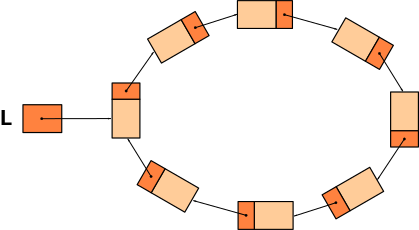
\includegraphics[scale=0.8]{../common-images/liste_variantes3_color.pdf}}
	\end{center}
%	\end{block}
\end{frame}


\begin{frame}[fragile=singleslide]
	\frametitle{Listes à fonctionnalités particulières}
	\begin{block}{}
		\begin{itemize}
			\item Limitation de l'accès aux éléments en fonction d'utilisations particulières (accès privilégié)
			\item \underline{Piles} (Last In First Out---LIFO)
			\item \underline{Files d'attentes} (First In First Out---FIFO)
		\end{itemize}
	\end{block}
\end{frame}


\begin{frame}[fragile=singleslide]
	\frametitle{Les piles}
	\begin{block}{Accès réduit : uniquement en tête}
		\begin{center}
			{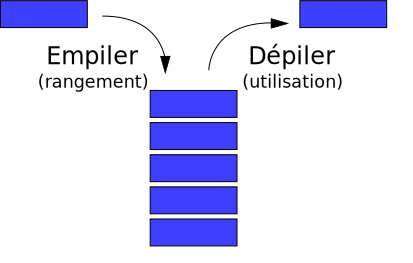
\includegraphics[scale=0.6]{../common-images/liste_variantes4.pdf}}
		\end{center}		
	\end{block}
	\vspace{-0.7cm}
	\begin{block}{Ordre chronologique inverse}
		\begin{columns}[c]
			\hspace{-0.5cm}
			\begin{column}{0.7\textwidth}
				\begin{itemize}
					\item Dernière information rangée
					\item Première utilisée
				\end{itemize}
			\end{column}
			%		\setlength{\columnseprule}{0.4pt}
			\hspace{-1.3cm}
			\vrule{}
			\hspace{0.3cm}
			\begin{column}{0.38\textwidth}
				\begin{center}
					\textbf{L}ast \textbf{I}n \textbf{F}irst \textbf{O}ut\\ \textbf{LIFO}
				\end{center}
			\end{column}
		\end{columns}
	\end{block}
\end{frame}



\begin{frame}[fragile=singleslide]
	\frametitle{Les piles: exemples}
	\begin{block}{}
		\begin{itemize}
			\item Pile de cartes
			\item Recherche d'un chemin sur une carte
			\begin{itemize}
				\item Aller de \texttt{i} en \texttt{j} : \texttt{empiler(i)}
				\item Revenir de \texttt{j} en \texttt{i} : \texttt{dépiler(i)}
				\item Quand la destination est rencontrée, le chemin recherché est dans la pile
			\end{itemize}
			\item Pile d'exécution de sous ­programmes
			\begin{itemize}
				\item Gérée automatiquement par le langage pour sauvegarder les contextes 
			d'exécution (restaurés dans l'ordre inverse des appels)
				\item Permet la récursivité
			\end{itemize}
		\end{itemize}
	\end{block}
\end{frame}



\begin{frame}[fragile=singleslide]
	\frametitle{Les piles: définition}
	\begin{block}{}
		\begin{itemize}
			\item \texttt{P : \underline{de type} Pile [de <T>]}
		\end{itemize}
	\end{block}
	\begin{block}{Opérations}
		\begin{itemize}
			\item \texttt{empiler(P,V)} : action qui ajoute un élément en sommet de pile
			\item \texttt{dépiler(P,V)} : action qui retire l'élément au sommet de pile et le range dans V
			\item \texttt{sommet(P)} : fonction qui retourne la valeur au sommet de pile sans la dépiler
			\item \texttt{pile\_vide(P)} : fonction qui teste si la pile est vide
		\end{itemize}
	\end{block}	
\end{frame}


%\begin{frame}[fragile=singleslide]
%	\frametitle{Les piles}
%	\begin{block}{}
%		\begin{itemize}
%			\item \texttt{init\_pile(P)} : action qui initialise la pile \texttt{P} à vide avant toute utilisation
%			\item \texttt{pile\_pleine(P)} : fonction qui teste si la pile est pleine (quand elle est de taille bornée)
%		\end{itemize}
%	\end{block}
%	\begin{block}{Remarques}
%		\begin{itemize}
%			\item \texttt{pile\_vide(P) $\Rightarrow$ sommet(P) } et \texttt{ dépiler(P,V)} invalides !
%			\item \texttt{pile\_pleine(P) $\Rightarrow$ empiler(P)} invalide !
%		\end{itemize}
%	\end{block}	
%\end{frame}

\begin{frame}[fragile=singleslide]
	\frametitle{Les piles}
	\begin{block}{}
		\begin{itemize}
			\item \texttt{init\_pile(P)} : action qui initialise la pile \texttt{P} à vide avant toute utilisation
			\item \texttt{pile\_pleine(P)} : fonction qui teste si la pile est pleine (quand elle est de taille bornée)
		\end{itemize}
	\end{block}
	\begin{block}{Operations Invalides}
		\begin{itemize}
			\item Si \hspace{0.2em} \texttt{pile\_vide(P) = Vrai} \hspace{0.2em} Alors
			\begin{itemize}
				\item[] \texttt{$\Rightarrow$} \sout{\texttt{sommet(P)}, \texttt{dépiler(P,V)}} \\sont invalides !
			\end{itemize}
			\item Si \hspace{0.2em} \texttt{pile\_pleine(P)=Vrai} \hspace{0.2em} Alors
			\begin{itemize}
				\item[] \texttt{$\Rightarrow$} \sout{\texttt{empiler(P)}} \\
				est invalide !
			\end{itemize}
			
		\end{itemize}
	\end{block}	
\end{frame}


\begin{frame}[fragile=singleslide]
	\frametitle{Les piles : choix d'implantation}
	\begin{block}{type abstrait $\rightarrow$ implantation}
		\begin{itemize}
			\item List dont on restreint l'accès
			\begin{itemize}
				\item chaînée
				\item contiguë
			\end{itemize}
		\end{itemize}
	\end{block}
\end{frame}


\begin{frame}[fragile=singleslide]
	\frametitle{Les piles : implantation par liste chaînée}
			\begin{center}
				\hspace{-0.83cm}
				{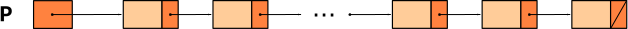
\includegraphics[scale=0.65]{../common-images/liste_variantes5.pdf}}
			\end{center}
	\begin{block}{}
		\begin{itemize}
			\item  \texttt{type Pile = Liste\_chaînée}
			\vspace{1em}
			\item[] {dépiler} $\longrightarrow$ \texttt{supp\_tête}
			\item[] {empiler} $\longrightarrow$ \texttt{ajout\_tête}
		\end{itemize}
	\end{block}
\end{frame}



\begin{frame}[fragile=singleslide]
	\frametitle{Les piles : implantation par liste chaînée}
	\begin{block}{}
		\begin{columns}[T]
			\hspace{-0.5cm}
			\begin{column}{0.7\textwidth}
				\begin{block}{Dépiler} %Gestion dynamique de la mémoire}
					\begin{minted}[mathescape=true,escapeinside=||,tabsize=4,fontsize=\footnotesize,]{c}
|\underline{Action}| dépiler(P, V)
	|\underline{D/R}| : P : Pile
	|\underline{R}| : V : <T>
	V |$\leftarrow$| P|$\uparrow$$\bullet$|valeur
	supp_tête(P)
|\underline{Faction}|
					\end{minted}
				\end{block}
				\begin{block}{Sommet} %Gestion dynamique de la mémoire}
					\begin{minted}[mathescape=true,escapeinside=||,tabsize=4,fontsize=\footnotesize,]{c}
|\underline{Fonction}| sommet(P) : <T>
	D : P : Pile
	Retourner (P valeur)
|\underline{Ffonction}|
					\end{minted}
				\end{block}
			\end{column}
			%		\setlength{\columnseprule}{0.4pt}
			\hspace{-1.3cm}
			\vrule{}
			\hspace{0.3cm}
			\begin{column}{0.38\textwidth}
				\begin{block}{Empiler} %Gestion dynamique de la mémoire}
					\begin{minted}[mathescape=true,escapeinside=||,tabsize=4,fontsize=\footnotesize,]{c}
|\underline{Action}| empiler(P, V)
	|\underline{D/R}| : P : Pile
	|\underline{D}| : V : <T>
	ajout_tête(P, V)
|\underline{Faction}|
					\end{minted}
				\end{block}		
			\end{column}
		\end{columns}
	\end{block}
\end{frame}

%
%\begin{frame}[fragile=singleslide]
%	\frametitle{Les piles : implantation par liste contiguë}
%	\begin{block}{}
%		\begin{itemize}
%			\item \texttt{sommet(P) : P.espace[P.dernier]}
%			\item \texttt{empiler(P, V) : P.dernier $\leftarrow$ P.dernier + 1}\\\texttt{P.espace[P.dernier] $\leftarrow$ V}
%			
%			\begin{columns}[T]
%%			\hspace{-0.5cm}
%				\begin{column}{0.7\textwidth}
%					\texttt{empiler(P, V) : P.dernier $\leftarrow$ P.dernier + 1}
%				\end{column}
%				%		\setlength{\columnseprule}{0.4pt}
%%				\hspace{-1.3cm}
%%				\vrule{}
%%				\hspace{0.3cm}
%				\begin{column}{0.38\textwidth}
%					\texttt{P.espace[P.dernier] $\leftarrow$ V}					
%				\end{column}
%			\end{columns}
%	
%%			\item dépiler(P, V) : V $\leftarrow$ P.espace[P.dernier]
%%			P.dernier $\leftarrow$ P.dernier ­ 1
%		\end{itemize}
%	\end{block}
%\end{frame}


\begin{frame}[fragile=singleslide]
	\frametitle{Les piles : implantation par liste contiguë}
	\begin{block}{}
		\begin{itemize}
			\item  \texttt{type Pile = Liste\_contiguë}
		\end{itemize}
	\end{block}	
	\begin{block}{Accès au dernier}
		\begin{minted}[mathescape=true,escapeinside=||,tabsize=4,
%		fontsize=\footnotesize
		,]{c}
sommet(P) :  P.espace[P.dernier]

empiler(P, V) : P.dernier |$\leftarrow$| P.dernier |$+$| 1
				P.espace[P.dernier] |$\leftarrow$| V
				
dépiler(P, V) : V |$\leftarrow$| P.espace[P.dernier]
				P.dernier |$\leftarrow$| P.dernier |$-$| 1
		\end{minted}
	\end{block}	
\end{frame}


\begin{frame}[fragile=singleslide]
	\frametitle{Les files d'attente}
	\begin{block}{}
		\begin{itemize}
			\item  Liste où les éléments sont utilisés dans l'ordre chronologique de leur rangement
		\end{itemize}
	\end{block}
		\begin{columns}[c]
			\hspace{-0.5cm}
			\begin{column}{0.7\textwidth}
				\begin{itemize}
					\item 1ère information rangée
					\item 1ère information traitée
				\end{itemize}
			\end{column}
			%		\setlength{\columnseprule}{0.4pt}
			\hspace{-1.3cm}
			\vrule{}
			\hspace{0.3cm}
			\begin{column}{0.38\textwidth}
				\begin{center}
					\textbf{F}irst \textbf{I}n \textbf{F}irst \textbf{O}ut\\ \textbf{FIFO}
				\end{center}
			\end{column}
		\end{columns}	
		\begin{center}
			\hspace{-0.83cm}
			{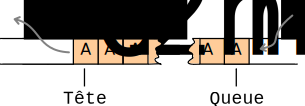
\includegraphics[scale=1]{../common-images/liste_variantes6.pdf}}
		\end{center}
\end{frame}


\begin{frame}[fragile=singleslide]
	\frametitle{Les files d'attente : exemples}
	\begin{block}{}
		\begin{itemize}
			\item Stock de données périssables
			\item Caisses de supermarché
			\item File d'attente de travaux d'impression sur imprimante de façon générale, file d'attente d'utilisation d'une ressource partagée
		\end{itemize}
	\end{block}
	\begin{block}{Définition du type}
		\begin{itemize}
			\item \texttt{F : \underline{file d'attente} de <T>}
			\item \texttt{F : \underline{FIFO} de <T>}
		\end{itemize}
	\end{block}
\end{frame}


\begin{frame}[fragile=singleslide]
	\frametitle{Les files d'attente : primitives}
	\begin{block}{}
		\begin{itemize}
			\item \texttt{init\_fifo(F)} : action qui initialise la FIFO \texttt{F} à vide (avant toute utilisation)
			\item \texttt{fifo\_vide(F) : booléen} : fonction qui teste si \texttt{F} est vide
			\item \texttt{fifo\_pleine(F) : booléen} : fonction qui test si F est pleine \{\textit{si la file est de taille bornée}\}
			\item \texttt{first(F) : <T>} : fonction qui rend la valeur de l'element de \texttt{F} sans l'extraire
			\item \texttt{put(F,X)} : action qui range \texttt{X} en queue de file
			\item \texttt{get(F,X)} : action qui extrait de la file l'élément de tête et le range dans \texttt{X}
		\end{itemize}
	\end{block}
\end{frame}


\begin{frame}[fragile=singleslide]
	\frametitle{Les files d'attente : implantation chaînée}
	\begin{block}{}
		\begin{itemize}
			\item Fortement dynamique
			\item Sans estimation aisée de la taille max
		\end{itemize}
	\end{block}
	\begin{block}{\texttt{get} et \texttt{first}}
		\begin{itemize}
			\item Accès en tête aisé au travers du pointeur de tête
		\end{itemize}
	\end{block}
	\begin{block}{\texttt{put} et \texttt{last}}
		\begin{itemize}
			\item Parcours séquentiel jusqu'au dernier : coûteux !!
			\item Besoin d'un accès privilégié en queue !
			\item Solution $\Rightarrow$ Maintenir un 2ème pointeur de queue
		\end{itemize}
	\end{block}
\end{frame}

\begin{frame}[fragile=singleslide]
	\frametitle{Les files d'attente : définition du type FIFO chaînée}
	\vspace{-0.83cm}
	\begin{block}{}
		\begin{minted}[mathescape=true,escapeinside=||,tabsize=4,
		%		fontsize=\footnotesize
		,]{c}
|\underline{type}| Ptcellule = |\underline{pointeur de}| Cellule

|\underline{type}| Cellule = structure
	valeur : <T>
	suivant : Ptcellule
|\underline{fin}|

|\underline{type}| Fifo = structure
	tête, queue : Ptcellule
|\underline{fin}|
		\end{minted}
	\end{block}
	\vspace{-0.5cm}	
	\begin{center}
		\hspace{-0.9cm}
		{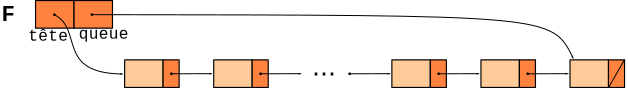
\includegraphics[scale=0.66]{../common-images/liste_variantes7.pdf}}
	\end{center}	
\end{frame}


\begin{frame}[fragile=singleslide]
	\frametitle{Les files d'attente : implantation chaînée}
	\begin{block}{}
		\begin{columns}[T]
			\hspace{-0.5cm}
			\begin{column}{0.7\textwidth}
				\begin{block}{Init} %Gestion dynamique de la mémoire}
					\begin{minted}[mathescape=true,escapeinside=||,tabsize=4,fontsize=\footnotesize,]{c}
|\underline{Action}| init_fifo(F)
	|\underline{D/R}| : F : Fifo |\underline{de}| <T>
	F.tête  |$\leftarrow$| NULL
	F.queue |$\leftarrow$| NULL
|\underline{Faction}|
					\end{minted}
				\end{block}
				\begin{block}{First} %Gestion dynamique de la mémoire}
					\begin{minted}[mathescape=true,escapeinside=||,tabsize=4,fontsize=\footnotesize,]{c}
|\underline{Fonction}| first(F) : <T>
	|\underline{D}| : F : Fifo |\underline{de}| <T>
	retourner(F.tête|$\uparrow$|.valeur)
|\underline{FFonction}|
					\end{minted}
				\end{block}
			\end{column}
			%		\setlength{\columnseprule}{0.4pt}
			\hspace{-3.5cm}
			\vrule{}
			\hspace{0.3cm}
			\begin{column}{0.38\textwidth}
				\begin{block}{Get} %Gestion dynamique de la mémoire}
					\begin{minted}[mathescape=true,escapeinside=||,tabsize=4,fontsize=\footnotesize,]{c}
|\underline{Action}| get(F, X)
	|\underline{D/R}| : F : Fifo |\underline{de}| <T>
	|\underline{R}| : X : <T>
	X |$\leftarrow$| F.tête|$\uparrow$|.valeur
	supp_tête(F.tête)
|\underline{Faction}|
					\end{minted}
				\end{block}		
			\end{column}
		\end{columns}
	\end{block}
\end{frame}


\begin{frame}[fragile=singleslide]
	\frametitle{Les files d'attente : implantation contiguë}
	\begin{block}{}
		\begin{itemize}
			\item Taille peu variable ou estimation aisée de \texttt{max}
			\item \texttt{put} et \texttt{last} :
			\begin{itemize}
				\item Accès en queue
				\item Aisé au travers de l'indice \texttt{queue}
			\end{itemize}
			\item \texttt{first} : accès en tête
			\item \texttt{get} :
			\begin{itemize}
				\item Compactage systématique : \textit{cher}
				\item Maintenir un indice \texttt{tete} et gérer un espace libre devant ?
				\item \underline{Solution} : boucler sur l'espace
			\end{itemize}
		\end{itemize}
	\end{block}
\end{frame}


\begin{frame}[fragile=singleslide]
	\frametitle{Les files d'attente : implantation contiguë}
	\begin{center}
		\hspace{-0.5cm}
		{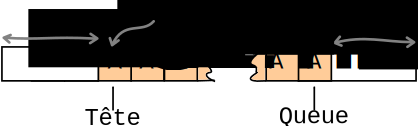
\includegraphics[scale=0.9]{../common-images/liste_variantes8.pdf}}
	\end{center}
	\begin{block}{Définition}
		\begin{minted}[mathescape=true,escapeinside=||,tabsize=4,
		%		fontsize=\footnotesize
		,]{c}
|\underline{type}| Fifo = |\underline{structure}|
  espace: vecteur [0..MAX-1] de <T>
  tete, queue: -1..MAX-1        |\footnotesize\{-1 si file vide\}|
|\underline{fin}|
		\end{minted}
	\end{block}
\end{frame}


\begin{frame}[fragile=singleslide]
	\frametitle{Les files d'attente : quelques primitives}
	\begin{block}{}
		\begin{columns}[T]
			\hspace{-2.2cm}
			\begin{column}{0.7\textwidth}
				\begin{block}{Init} %Gestion dynamique de la mémoire}
					\begin{minted}[mathescape=true,escapeinside=||,tabsize=4,fontsize=\footnotesize,]{c}
|\underline{Action}| init_fifo(F)
	|\underline{D/R}| : F : Fifo |\underline{de}| <T>
	F.queue |$\leftarrow$| -1
	F.tete |$\leftarrow$| -1
|\underline{Faction}|
					\end{minted}
				\end{block}
				\begin{block}{Vide} %Gestion dynamique de la mémoire}
					\begin{minted}[mathescape=true,escapeinside=||,tabsize=2,fontsize=\footnotesize,]{c}
|\underline{Fonction}| fifo_vide(F): booléen
	|\underline{D}| : F : Fifo |\underline{de}| <T>
	retourner(F.tete = -1)
|\underline{FFonction}|
					\end{minted}
				\end{block}
			\end{column}
			%		\setlength{\columnseprule}{0.4pt}
			\hspace{-4.25cm}
			\vrule{}
			\hspace{0cm}
			\begin{column}{0.38\textwidth}
				\begin{block}{Pleine} %Gestion dynamique de la mémoire}
					\begin{minted}[mathescape=true,escapeinside=||,tabsize=2,fontsize=\footnotesize,]{c}
|\underline{Fonction}| fifo_pleine(F): booléen
	|\underline{D}| : F : Fifo |\underline{de}| <T>
	retourner(
		F.tete = (F.queue+1) mod MAX
	)
|\underline{FFonction}|
					\end{minted}
				\end{block}
				\begin{block}{First} %Gestion dynamique de la mémoire}
					\begin{minted}[mathescape=true,escapeinside=||,tabsize=4,fontsize=\footnotesize,]{c}
|\underline{Fonction}| first(F) : <T>
	|\underline{D}| : F : Fifo |\underline{de}| <T>
	retourner(F.espace[F.tete])
|\underline{FFonction}|
					\end{minted}
				\end{block}		
			\end{column}
		\end{columns}
	\end{block}
\end{frame}


\begin{frame}[fragile=singleslide]
	\frametitle{Les files d'attente : implantation contiguë\\ \texttt{put}}
	\begin{block}{}
		\begin{minted}[mathescape=true,escapeinside=||,tabsize=4,
		%		fontsize=\footnotesize
		,]{c}
|\underline{Action}| put(F, X)
	|\underline{D/R}| : F : Fifo |\underline{de}| <T>
	|\underline{D}| : X : <T>
	
	{valide si fifo_pleine(F) |$\neq$| faux}

	|\underline{Si}| F.queue = -1 |\underline{Alors}|
		F.tete = 0
	|\underline{Fsi}|

	F.queue |$\leftarrow$| (F.queue+1) mod MAX
	F.espace[F.queue] |$\leftarrow$| X
|\underline{Faction}|
		\end{minted}
	\end{block}
\end{frame}


\begin{frame}[fragile=singleslide]
	\frametitle{Les files d'attente : implantation contiguë\\ \texttt{get}}
	\vspace{-0.4cm}
	\begin{block}{}
		\begin{minted}[mathescape=true,escapeinside=||,tabsize=4,
		%		fontsize=\footnotesize
		,]{c}
|\underline{Action}| get(F, X)
	|\underline{D/R}| : F : Fifo |\underline{de}| <T>
	|\underline{R}| : X : <T>

	{valide si fifo_vide(F) |$\neq$| faux}

	X |$\leftarrow$| F.espace[F.tete]

	|\underline{Si}| F.tete = F.queue |\underline{Alors}|
		F.tete |$\leftarrow$| F.queue |$\leftarrow$| -1
	|\underline{Sinon}|
		F.tete |$\leftarrow$| (F.tete+1) mod MAX
	|\underline{Fsi}|
|\underline{Faction}|
		\end{minted}
	\end{block}
\end{frame}

% % % % % % % % % % % % % % % % % % % % % % % % % % %
% END
% % % % % % % % % % % % % % % % % % % % % % % % % % %
\end{document}
% % % % % % % % % % % % % % % % % % % % % % % % % % %
% END
% % % % % % % % % % % % % % % % % % % % % % % % % % %